\chapterimage{back2.jpg} % Chapter heading image
\chapter{Programming}

\section{Installation}

The starter kit SK$_0$ is composed of: 
\begin{itemize}
    \item The CLEARSY Safety Platform board
    \item A micro-USB connector to upload the software and to monitor its execution
    \item A power supply
    \item 3 switches connected to the 3 digital inputs I$_1$, I$_2$ and I$_3$
    \item The development environment running on Windows
    \item The user manual (this book)
\end{itemize}

\begin{figure}[ht]
\centering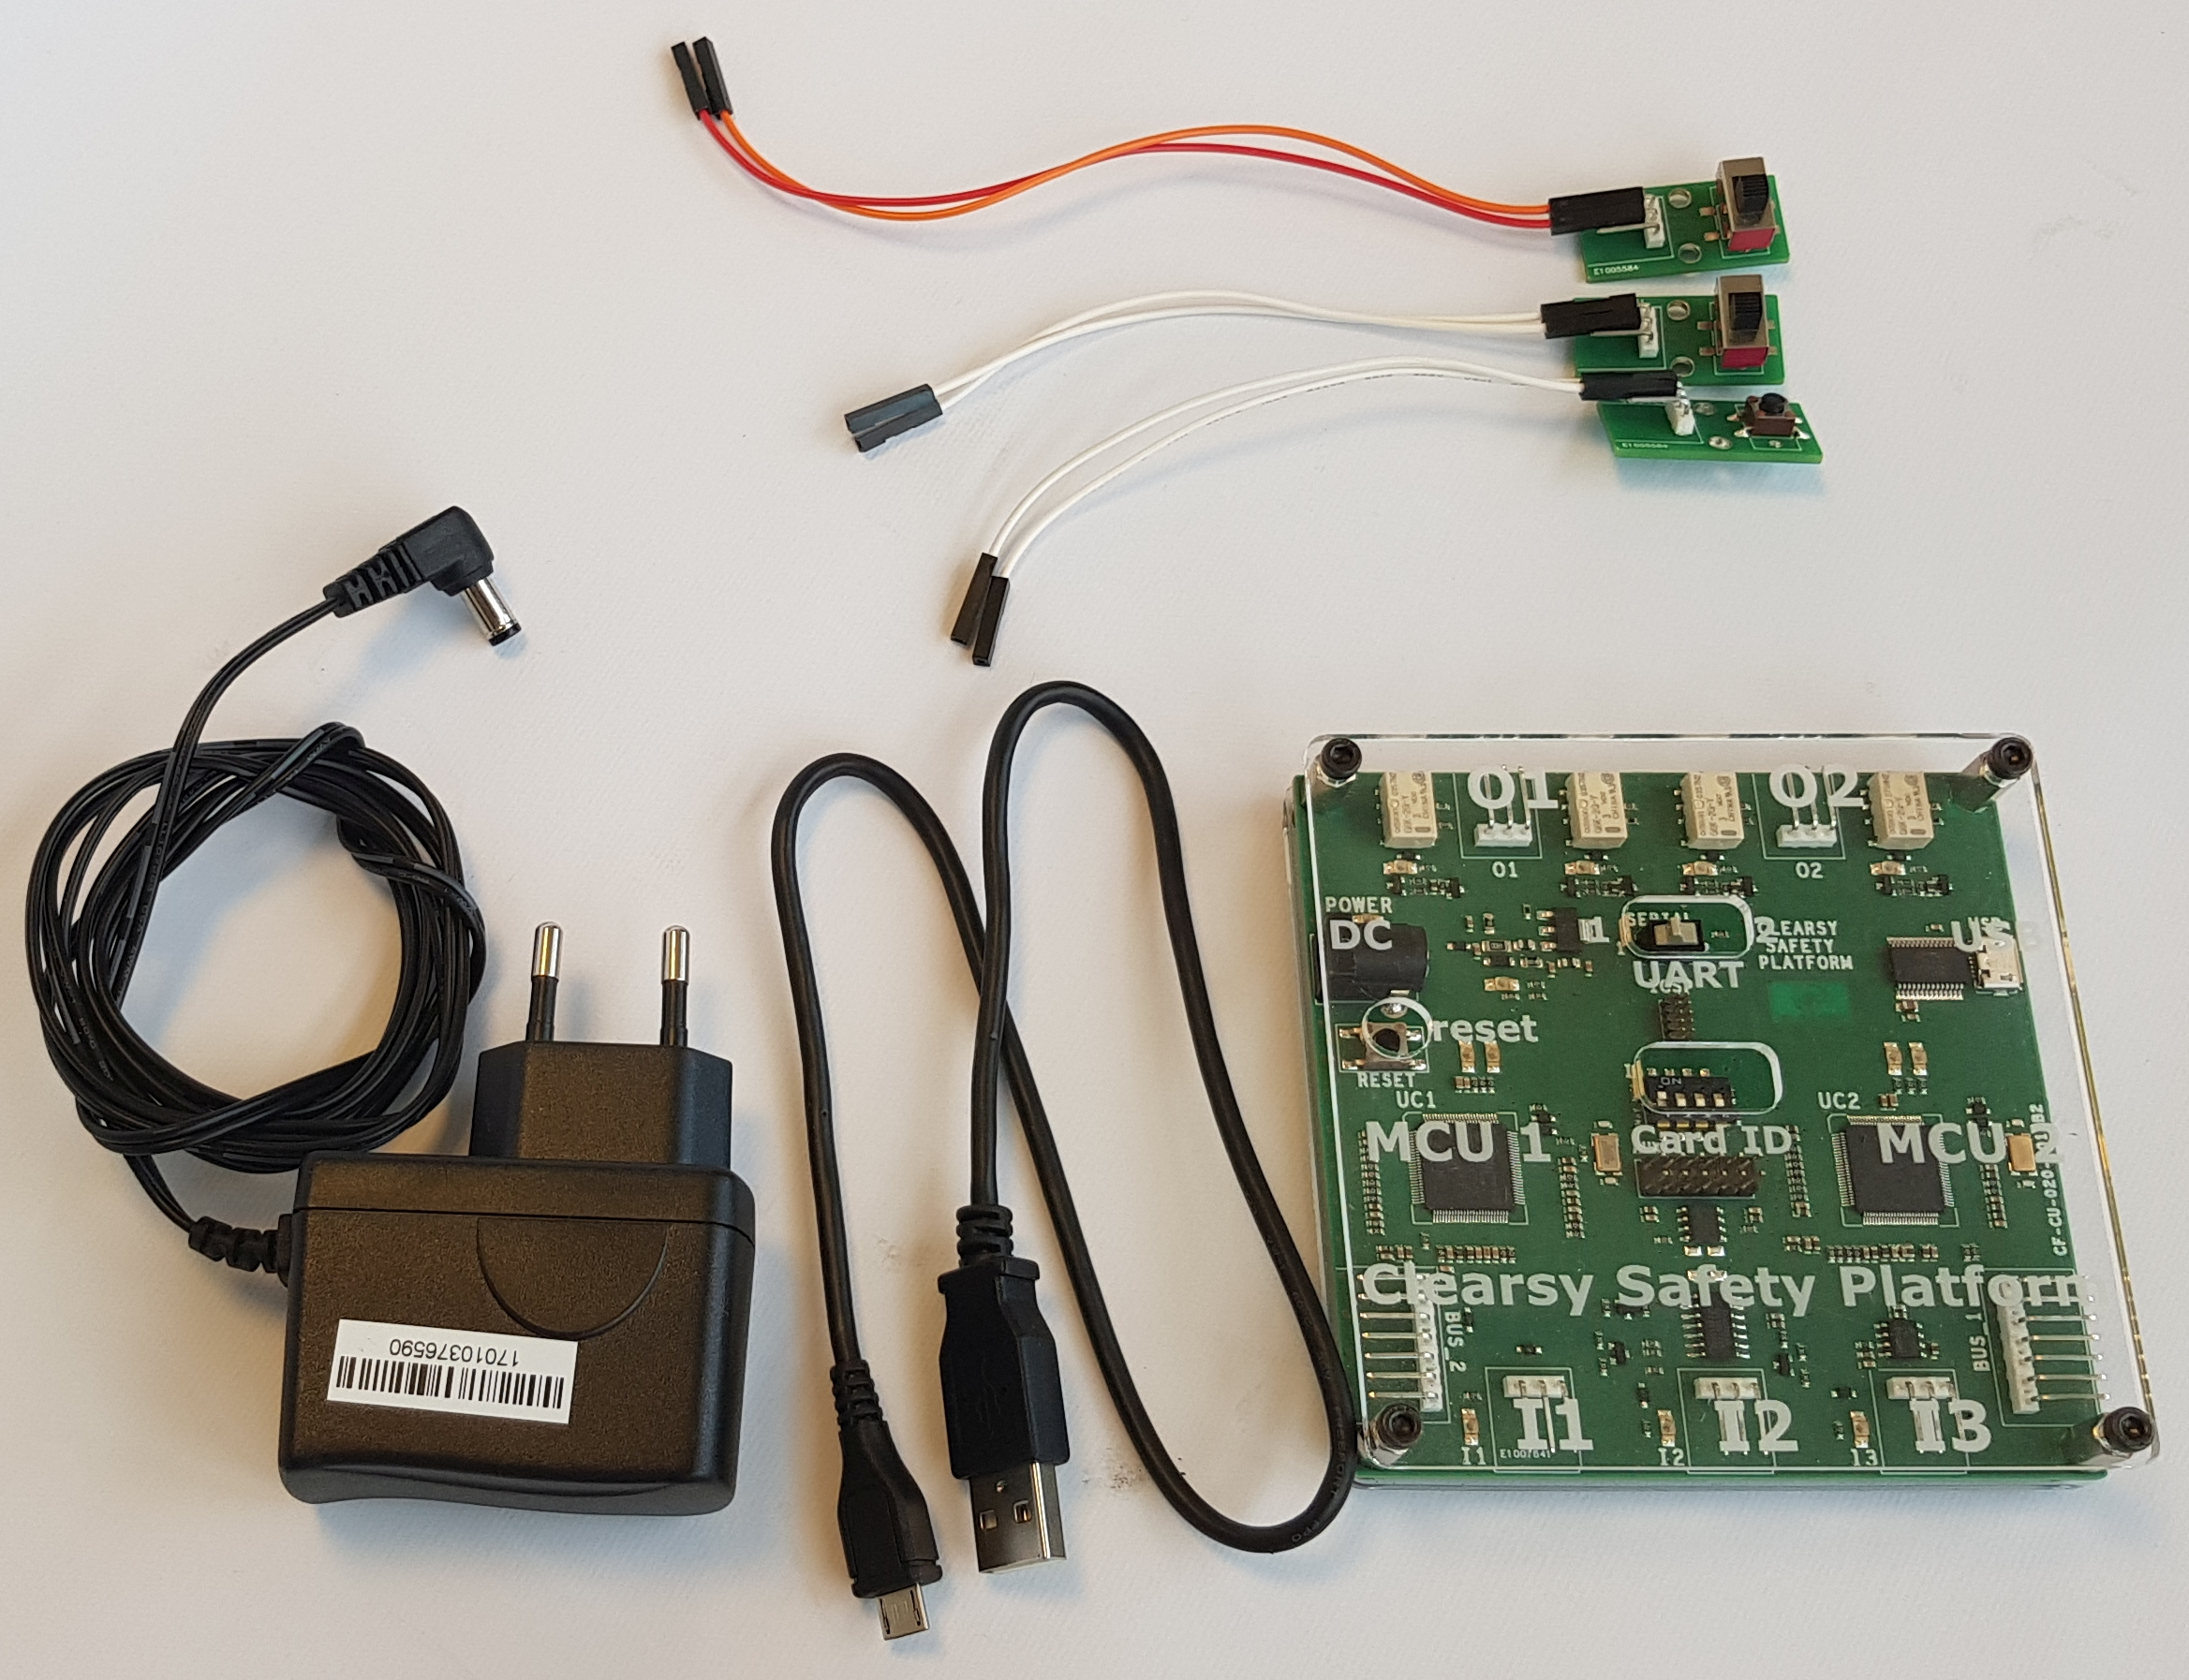
\includegraphics[scale=0.09]{Pictures/chapterProgramming/INSTALL-SK0.jpg}
\caption{The CLEARSY Safety Platform starter kit 0}
\label{install:SK0}
\end{figure}

\begin{remark}
Warning ! Do not connect the board to your PC before having completed the installation of the FTDI driver. Sometimes Windows installs another (inadequate) driver that prevents any further communication with the board. Then removing this driver is mandatory before installing the FTDI driver.
\end{remark}

The installation of the development environment is as follow:
\begin{itemize}
    \item download the installer file containing the IDE \footnote{When you buy a CSSP starter kit, you receive by email a link to download the IDE.}. The file is around 0.4 GB. 
    \item execute the installer and install it to a directory. It requires 3 GB of free space on your hard disk.  Choose preferably a path which does not contains spaces or special characters. 
        \item install the FTDI driver. Execute the file CDM21228\_Setup.exe in the directory "Drivers \& runtime". This driver is required to emulate the CSSP serial port over USB in order to communicate with the board (upload, monitor).
\end{itemize}  

\begin{figure}[ht]
\centering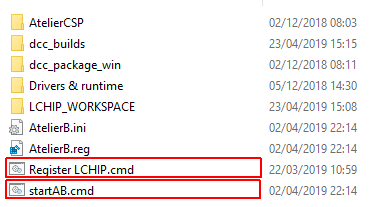
\includegraphics[scale=0.5]{Pictures/chapterProgramming/INSTALL-directory.png}
\caption{The directory where the IDE has been installed. The two scripts to use for respectively configuring and starting the IDE are highlighted in red. Register LCHIP.cmd is executed automatically during installation. startAB.cmd launches the CSSP IDE.}
\label{install:directory}
\end{figure}



\section{A first run}
During this first run, we are going to experiment with the full process of programming the CLEARSY Safety Platform. Let us start by executing the startAB.cmd script to verify that the installation has been completed. You should obtain the window shown in the figure \ref{install:ATB-window} with the two projects \textit{Clock} and \textit{Combinatorial} listed in the left pane.

\begin{figure}[h]
\centering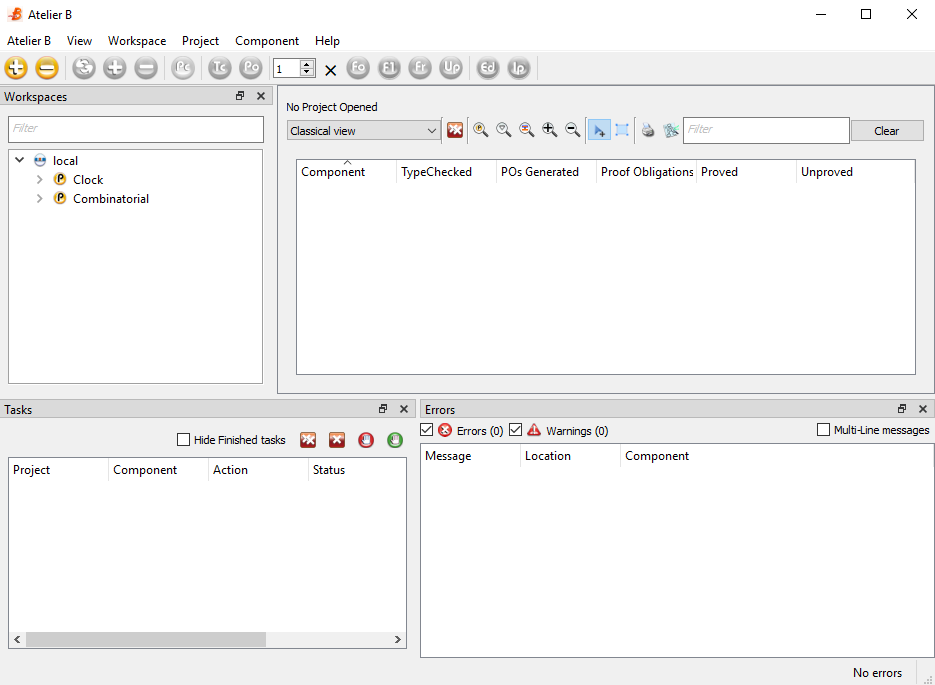
\includegraphics[scale=0.35]{Pictures/chapterProgramming/INSTALL-ATB-window.png}
\caption{The Atelier CSSP main window when executing the startAB.cmd script}
\label{install:ATB-window}
\end{figure}

\begin{remark}
\textbf{Troubleshooting}\\
If the two projects \textit{Clock} and \textit{Combinatorial} do not show up on the project list pane (left), you probably  do not have the rights to modify the Atelier B configuration files in the directory press/bdb.
\end{remark}
Power the board by using the power supply. Connect the CLEARSY Safety Platform to your PC with a micro-USB cable.  The board should now have some LEDs on after few seconds. The board is executing the program that was previously uploaded in memory. If it is the very first use of the board, the flash memory is empty and the board is literally doing nothing.\\
Let us create our first CLEARSY Safety Platform project:
\begin{itemize}
    \item go to the menu Atelier B / New / Project.
    \item select "Software development" and "Define as CSSP project" (figure \ref{install:create-project}).
    \item enter a project name that is not yet defined in the project list pane
\end{itemize}

\begin{figure}[ht]
\centering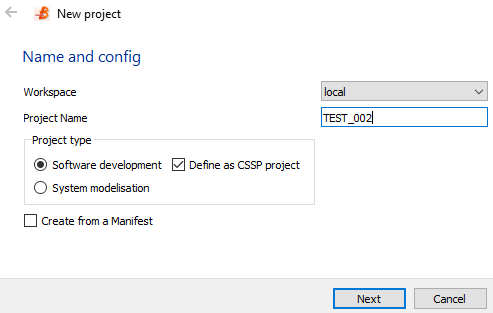
\includegraphics[scale=0.4]{Pictures/chapterProgramming/FIRSTRUN-create-project-001.png}
\caption{Information required to create a CSSP project}
\label{install:create-project}
\end{figure}

\begin{itemize}    
    \item click "Next" then "Finish".
    \item a new window requires you to select the board type - keep the default choice "SK0" and press "OK".
    \item a new window shows up to configure the number and names of the IOs.
    \item click on "create new board".
    \item a graphical representation of the board appears together with two panes on the right that allow to select the inputs to use and to edit their default name (figure \ref{install:configure-board}).
\end{itemize}
  
  \begin{figure}[h]
\centering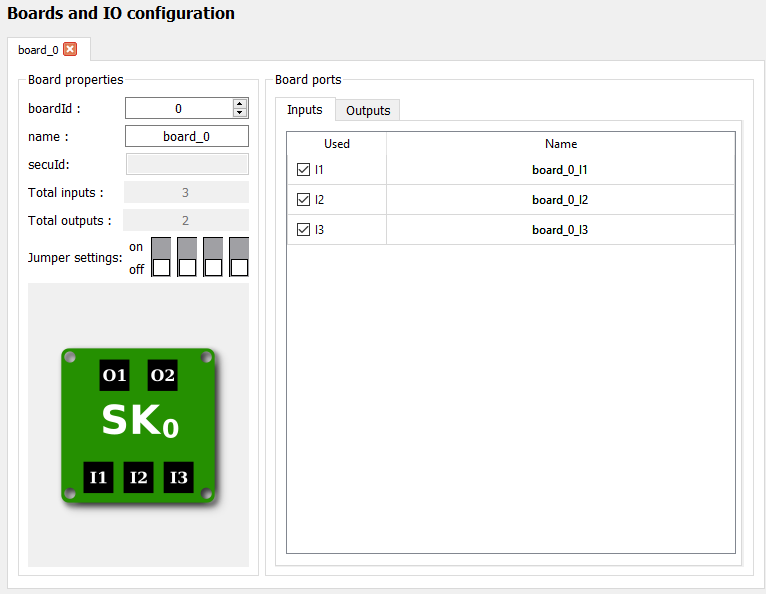
\includegraphics[scale=0.3]{Pictures/chapterProgramming/FIRSTRUN-create-project-004.png}
\caption{The configuration window to select the inputs/outputs and to modify the default naming}
\label{install:configure-board}
\end{figure}  
    
\begin{itemize}
    \item once your are happy with the configuration, click "Next".
    \item a summary page is displayed with the exact configuration of the board.
    \item click on "Finish" - you are asked to confirm the writing of the configuration. As we are creating the project, there is no previous configuration, so we can safely save it. Click on "Yes".
    \item the components of the project are generated in few seconds.
    \item then you finally get several orange boxes in the main window. The boxes represent the components generated from the configuration (IOs numbers and names). The colour represents their proof status: red/orange is "not proved", green is "proved" (figure \ref{install:project-components}).
 \end{itemize}
  
  \begin{figure}[h]
\centering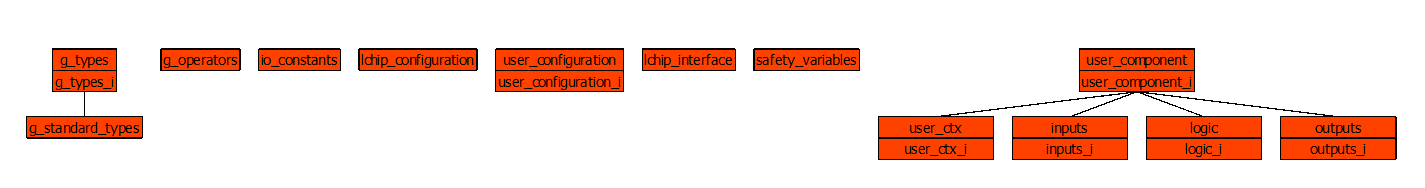
\includegraphics[scale=0.28]{Pictures/chapterProgramming/FIRSTRUN-create-project-005.png}
\caption{The CSSP project generated from the board configuration. Boxes are components.}
\label{install:project-components}
\end{figure}  
    
\begin{itemize}   
    \item select all the components with Ctrl-A.
    \item initiate their proof with Ctrl-0 (or click on the blue button "F0" on the toolbar).
    \item within 30 seconds, all the components turn to green. The project is completely proved. 
    \item now that the correctness of the project is ensured, we need to compile it. Right click on the project name (left pane) and select "CSSP Runner"\footnote{there is also a "CSSP Runner SK1" to use only with the board SK1.}.
    \item a new window - the CSSP runner - shows up, representing graphically the different stages of the compilation (figure \ref{install:cssp-runner}).
\end{itemize}
  
  \begin{figure}[ht]
\centering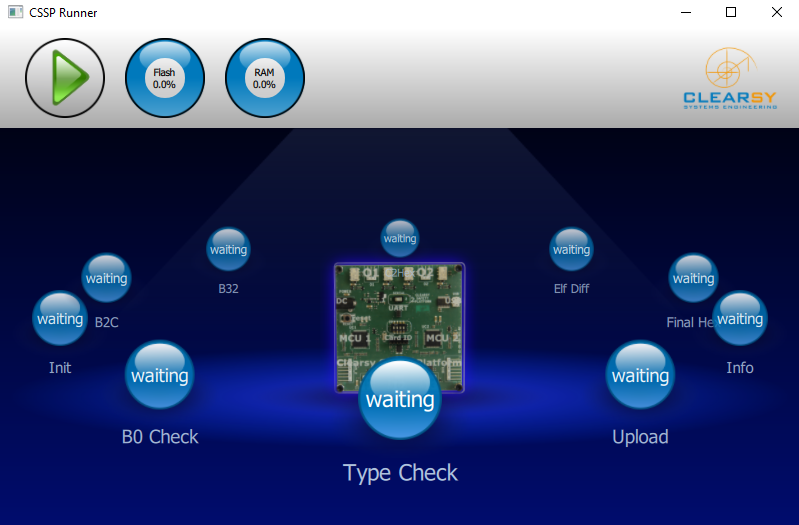
\includegraphics[scale=0.4]{Pictures/chapterProgramming/FIRSTRUN-create-project-006.png}
\caption{The CSSP runner shows the different stages of the compilation process}
\label{install:cssp-runner}
\end{figure}  
    
\begin{itemize}    
    
    \item click the green triangle on the top left to initiate the compilation
    \item an animation shows how the different stages are completed with (normally) a green tick for all of these. The memory footprint is displayed on the top during the penultimate stage. 
    \item finally the runner reaches the last stage - upload. You are asked to reset the SK0 board. Push on the reset button on the board; the board starts blinking as it enters the bootload mode \footnote{This mode is used to modify the program in flash.} and downloads the program.
    \item once the transfer is completed, you are asked to reset the board again, to leave the bootload mode. The program in flash is copied in memory then its execution is initiated.
    \item the program does nothing (no modification of the outputs): so normally you should observe the two outputs O1 and O2 of the boards set to OFF (LEDs off), and the board status LED blinking slowly. 
\end{itemize}
Congratulations! You have successfully programmed the SK0 board for the first time!

%-------------------------------------------------
\section{The programming model}

The CLEARSY Safety Platform is aimed at \textbf{automation functions for cyclic applications}, as it 
\begin{itemize}
    \item reads the digital inputs.
    \item performs computations using a subset of the B language.
    \item modifies the outputs.
    \item reads the current time since the central unit started.
\end{itemize}
The function is executed regularly as often as possible similar to Arduino programming (setup(), loop()). 
  \begin{figure}[ht]
\centering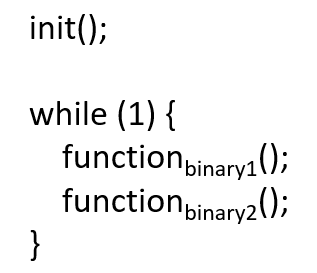
\includegraphics[scale=0.3]{Pictures/chapterProgramming/main-loop-pseudo-code.png}
\caption{The pseudo-code of the main loop}
\end{figure}  
There is no underlying operating system and no interrupt. 
There is no delay(). There is no predefined cycle time. However if the outputs are not set and cross-read every 50 ms, the board SK$_0$ enters panic mode and reboots.\\
Inputs are values captured at the beginning of a cycle (instantaneous values). Input capture is synchronised on both microcontrollers in order to acquire the same values (and prevent unwanted reboot because of different behaviour over the two central units). Outputs are maintained from one cycle to another.\\

With the CLEARSY Safety Platform, the developer is incited to focus on developing a function, independently of its transformation and distributed execution. 

%-------------------------------------------------
\section{Development cycle: the steps}

The CSSP development cycle strictly follows the B method which can be summarised as:
\begin{itemize}
    \item specification model is written first, then comes the implementation model, both using the same language (B).
    \item models are proved.
    \item source code is generated from implementation models.
\end{itemize}
The whole picture (figure \ref{programming:b-method}) contains more details that are going to be explained. Fortunately the CSSP IDE helps to lower the number of actions to perform when developing an application.
  \begin{figure}[ht]
\centering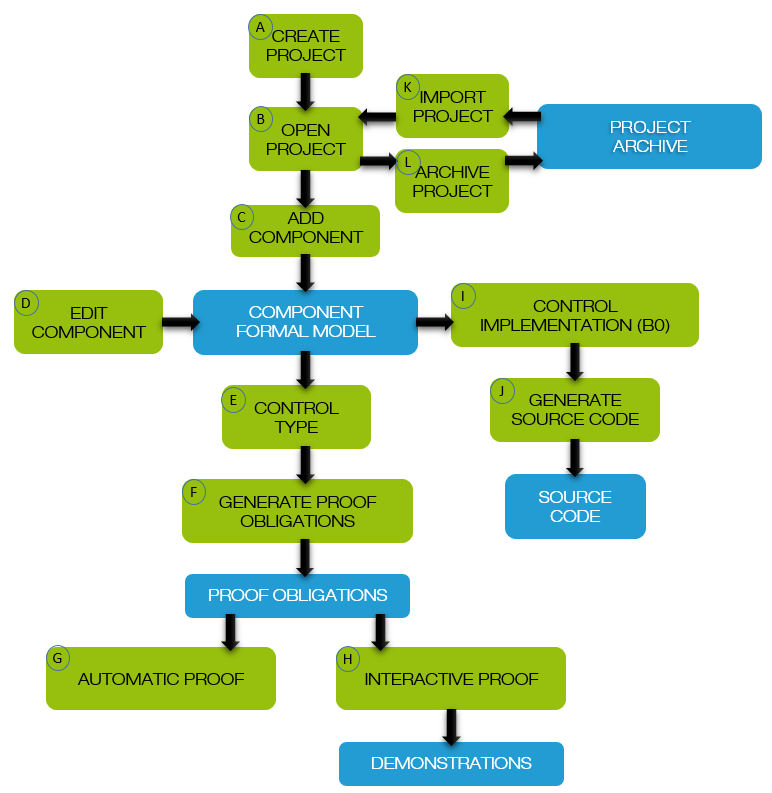
\includegraphics[scale=0.4]{Pictures/chapterProgramming/b-method.png}
\caption{The development cycle with the B method - blue boxes are files, green ones are actions performed with the CSSP IDE.}
\label{programming:b-method}
\end{figure}  

\subsection{CSSP project creation}

Creating a CSSP project\footnote{A software development project + CSSP option} covers actions \circled{A}, \circled{B}, and \circled{C}. The project is created and populated with the required components (§ \ref{annexes:interface-with-safety-library}) based on your board configuration (number and naming of inputs and outputs). There is no need to add other components for simple applications. 
\begin{remark}
It is not possible to regenerate a project once it has been created from a given configuration, in case for example you made a spelling mistake that you want to correct. As the components are automatically generated, you are going to loose all edits. Just create another project and copy/paste your edits from one project to the other.
\end{remark}

\subsection{Editing CSSP components}

Editing CSSP components covers action \circled{D}. You are entitled to modify the following components:
\begin{itemize}
    \item \textbf{user\_ctx} by 
    \begin{itemize}    
        \item adding constants (clause CONCRETE\_CONSTANTS) (optional),
        \item providing properties defining constants' types and constraints (clause PROPERTIES),
        \item adding sets (clause SETS) (optional).
    \end{itemize}   
    \item \textbf{user\_ctx\_i} by providing values to your concrete constants and sets (clause VALUES)
    \item \textbf{user\_logic} by modifying the specification of the operation user\_logic. By default, the specification is skip, meaning that all variables defined at specification level are not modified. 
    \item \textbf{user\_logic\_i} by 
    \begin{itemize}    
        \item adding variables (clause CONCRETE\_VARIABLES) (optional),
        \item adding typing properties for variables (clause INVARIANT) ,
        \item adding initialisation values for variables (clause INITIALISATION),
        \item modifying the body of the operation user\_logic (clause OPERATIONS).
    \end{itemize}   
\end{itemize}

\subsection{Proving CSSP project}

Proving CSSP project covers actions \circled{E}, \circled{F}, and \circled{G}. Initiating automatic proof by selecting one/several/all components and clicking on the "F0" button on the toolbar will start automatic proof in force 0 of these components. If required, type control and proof obligation generation are performed automatically. Your project is fully proved if all component boxes are green with graphical view or 100\% proved with classical view (figure \ref{programming:proof-status-classical}).

  \begin{figure}[ht]
\centering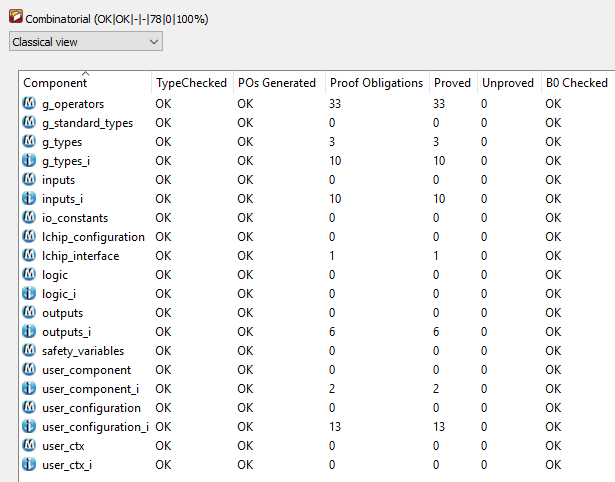
\includegraphics[scale=0.4]{Pictures/chapterProgramming/project-status-classical.png}
\caption{Proof status with classical view: 100\% proved requires to have only zeros in the "Unproved" column.}
\label{programming:proof-status-classical}
\end{figure}  

\subsection{Interactively proving  CSSP project}

Interactively proving CSSP project covers action \circled{H}. A project not fully proved automatically does not necessarily mean that the project contains errors. Unproved proof obligations might be not "adequate"/too complicated for the proof tools and require some guidance from the developer to complete the mathematical demonstration like starting a proof by contradiction or by cases, rewriting/simplifying predicates/expressions, etc. Interactive proof is an advanced topic and as such will be addressed later. 

\subsection{Generating code for CSSP project}

Generating code for CSSP project covers actions \circled{I} and \circled{J}. The CSSP Runner is triggered by selecting the project, right-clicking and then by clicking "CSSP Runner" in the drop-down menu. A new window shows up with a rotating view of the different compilation steps. After clicking the green triangle button on the top left, the different stages are executed. 
\begin{itemize}
    \item If a stage fails, you get a red cross and the compilation process stops (figure \ref{programming:runner-error}). If you click on the "error" text, you get the logs captured during the execution of the related tool. These logs may be copied by right clicking and selecting the action "copy" from the drop-down menu. 
\end{itemize}    
      \begin{figure}[h]
\centering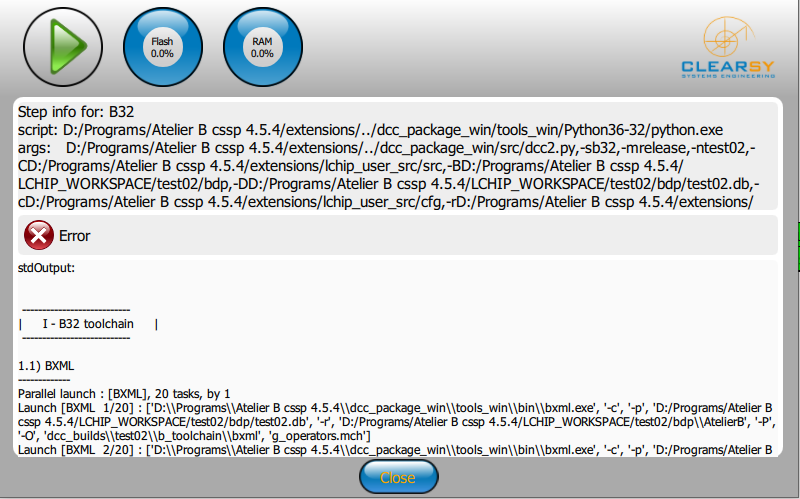
\includegraphics[scale=0.3]{Pictures/chapterProgramming/runner-error.png}
\caption{Clicking on the Error displays the logs captured during the execution of the related tool.}
\label{programming:runner-error}
\end{figure}  
\begin{itemize}
    \item If all the compilation stages succeed, you get information about the memory consumption for both Flash and RAM. Check that you do not reach 100\%. You are asked to reset the board to enter bootload mode. As soon as the reset button is pushed, the two upload LEDs start blinking for around 30 seconds. Then the last stage gets a green tick and you are asked to reset again the board to leave bootload mode. Once the reset button is pressed, the board starts executing the software copied in Flash memory within 2 seconds.
\end{itemize}
      \begin{figure}[h]
\centering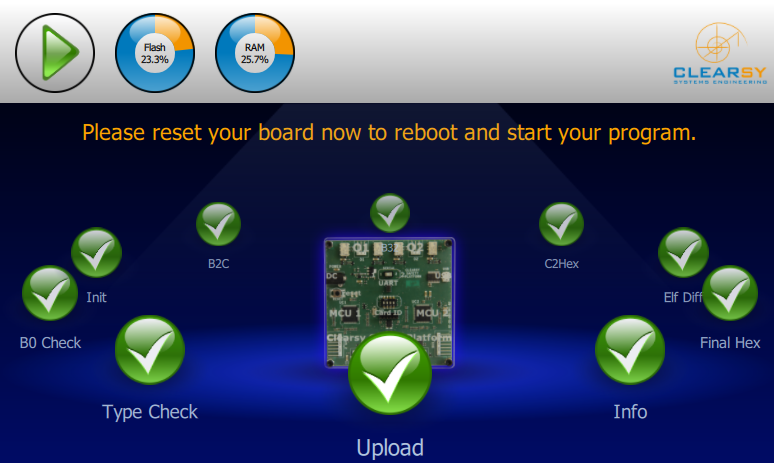
\includegraphics[scale=0.3]{Pictures/chapterProgramming/runner-upload-completed.png}
\caption{All green ticks indicate a successful compilation and upload.}
\label{programming:runner-upload-completed}
\end{figure}  

\subsection{Archiving and importing for CSSP project}

Archiving and importing for CSSP project cover actions \circled{K} and \circled{L}. To archive a project, select it, right-click and select "archive". Chose the destination directory (the archive file has the .arc extension). Chose "whole project" then "Next" and "Finish".
To import a CSSP project, select "Workspace/restore project". Click "Next". Select the archive file to you to import, give a name to the project and click "Next" then "Finish". A new project appears in the left pane, with the contents of the archived project.

%-------------------------------------------------
\section{Programming the board}

Programming the board (figure \ref{programming:all})  consists of:
\begin{itemize}
    \item describing, in the component \textit{logic}, the behaviour of the board,
    \item declaring and using constants, defined in the component \textit{user\_ctx},
    \item reusing operations defined in the component \textit{inputs} and in the safety library.
\end{itemize}
\begin{figure}[ht]
\centering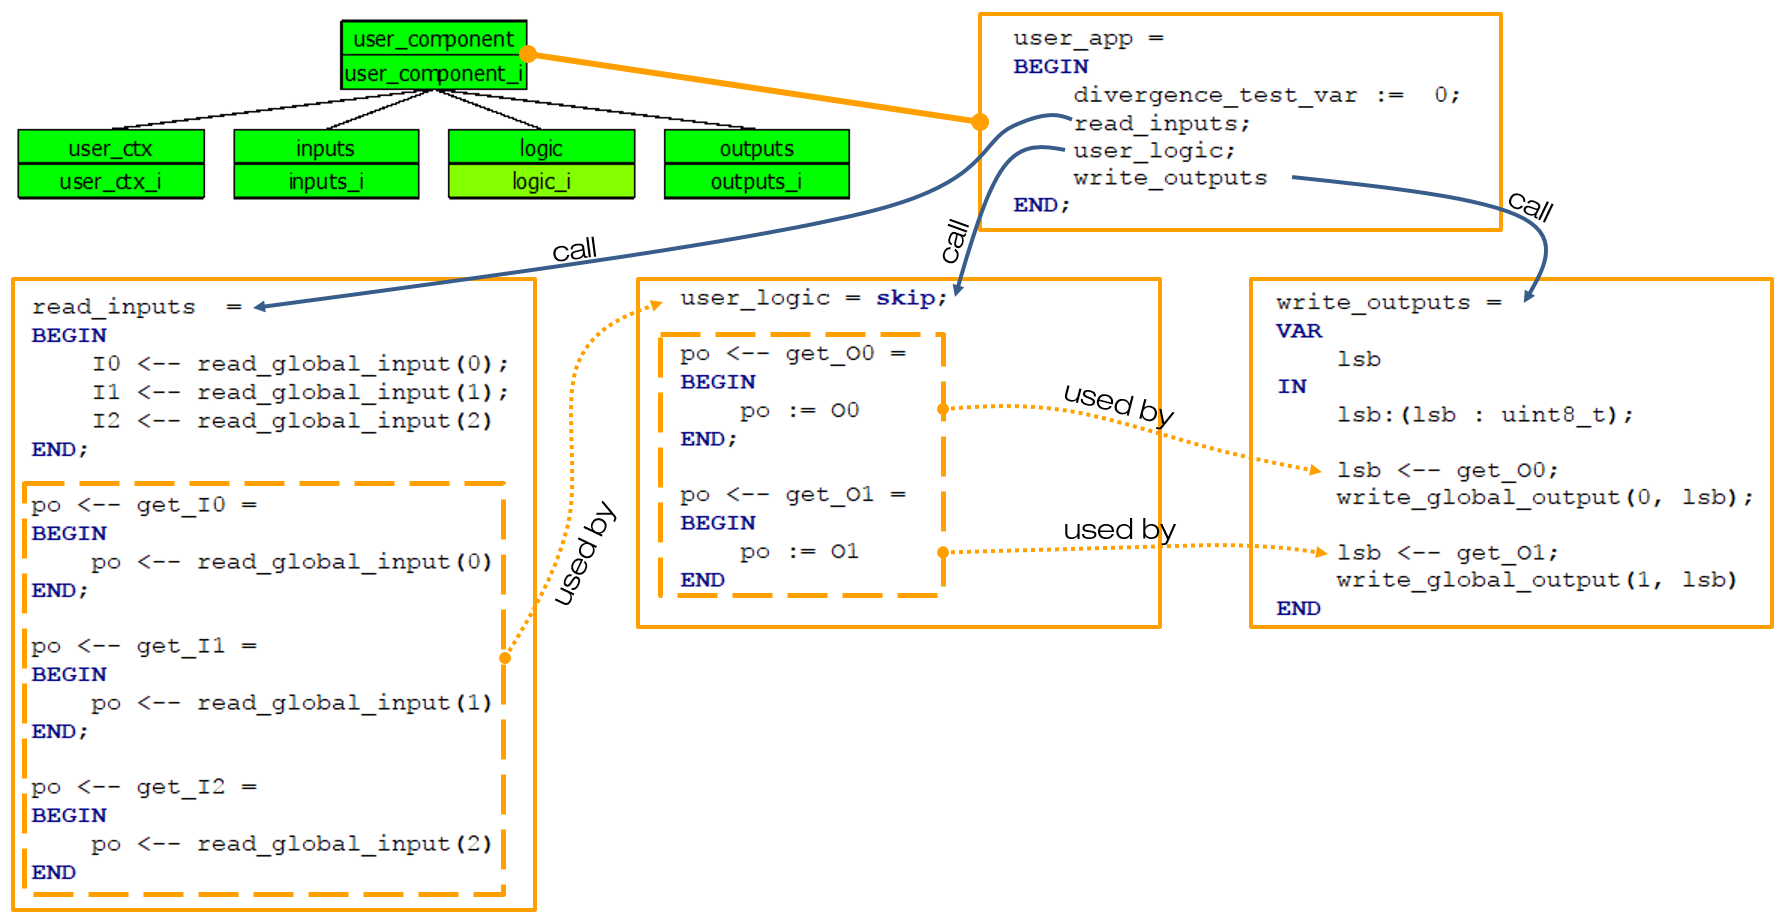
\includegraphics[scale=0.25]{Pictures/chapterProgramming/programming-all.png}
\caption{The default CSSP project showing the dependencies between the components. }
\label{programming:all}
\end{figure} 
All the operations defined in the components \textit{inputs} and \textit{outputs} have to remain unchanged, as well as the accessing functions get\_* defined in the component \textit{logic}.\\
The structure of the component \textit{logic} is seen in figure \ref{programming:spec}. It contains several clauses:
\begin{itemize}
    \item SEES: contains the list of all seen components.
    \item ABSTRACT\_VARIABLES: the outputs of the board. They are going to be refined in CONCRETE\_VARIABLES (implementable) in the component \textit{logic\_i}.
    \item INVARIANT: the type of the variables, with some constraints between them (optional).
    \item INITIALISATION: the first value assigned to the variables. At specification level, initialisation may be non-deterministic (any value complying with some conditions).
    \item OPERATIONS: each operation specifies how the modelling variables are modified, preferably without the algorithmic details.
\end{itemize}
\begin{figure}[ht]
\centering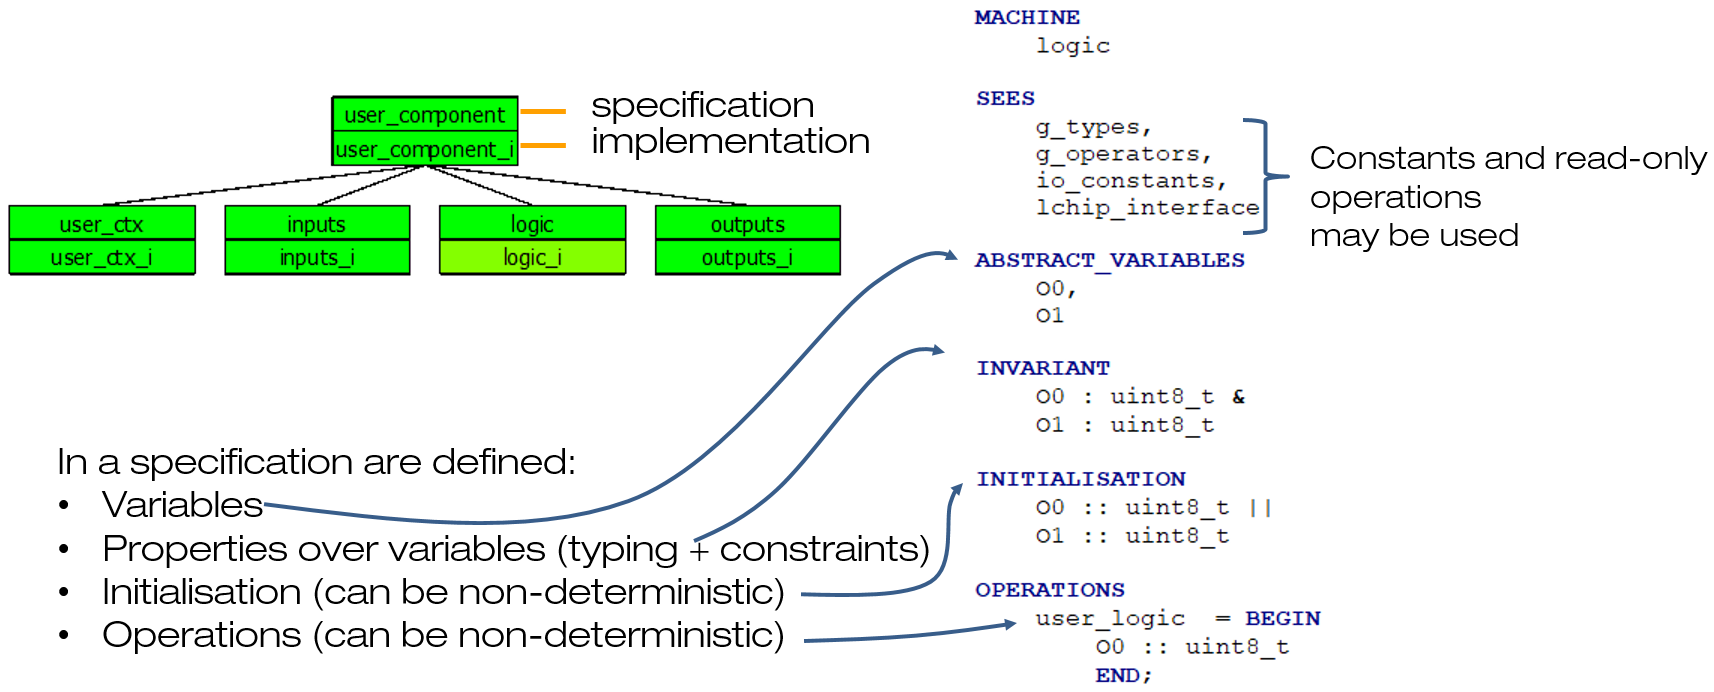
\includegraphics[scale=0.25]{Pictures/chapterProgramming/programming-spec.png}
\caption{The structure of the \texit{logic} component (specification).}
\label{programming:spec}
\end{figure}
Once the specification component has been modified\footnote{It should mention \textit{a minima} that the outputs are going to be modified when the operation user\_logic is executed.}, it is time to modify the component \textit{logic\_i}. 
The structure of the component \textit{logic\_i} (figure \ref{programming:implem}) is quite similar to that of component \textit{logic}:
\begin{itemize}
    \item SEES: the implementation should see the same components.
    \item CONCRETE\_VARIABLES: outputs variables have to be concrete (implementable). New variables (not defined in the component \textit{logic}) could be added.
    \item INVARIANT: a concrete type (uint8\_t, uint16\_t, uint32\_t, or BOOL) has to be given to all concrete variables declared. Board outputs must be declared as uint8\_t.
    \item INITIALISATION: all variables have to be assigned a deterministic value. This value should comply with its type.
    \item OPERATIONS: the behaviour of each operation has to be implemented with only implementable substitutions.
\end{itemize}
\begin{figure}[ht]
\centering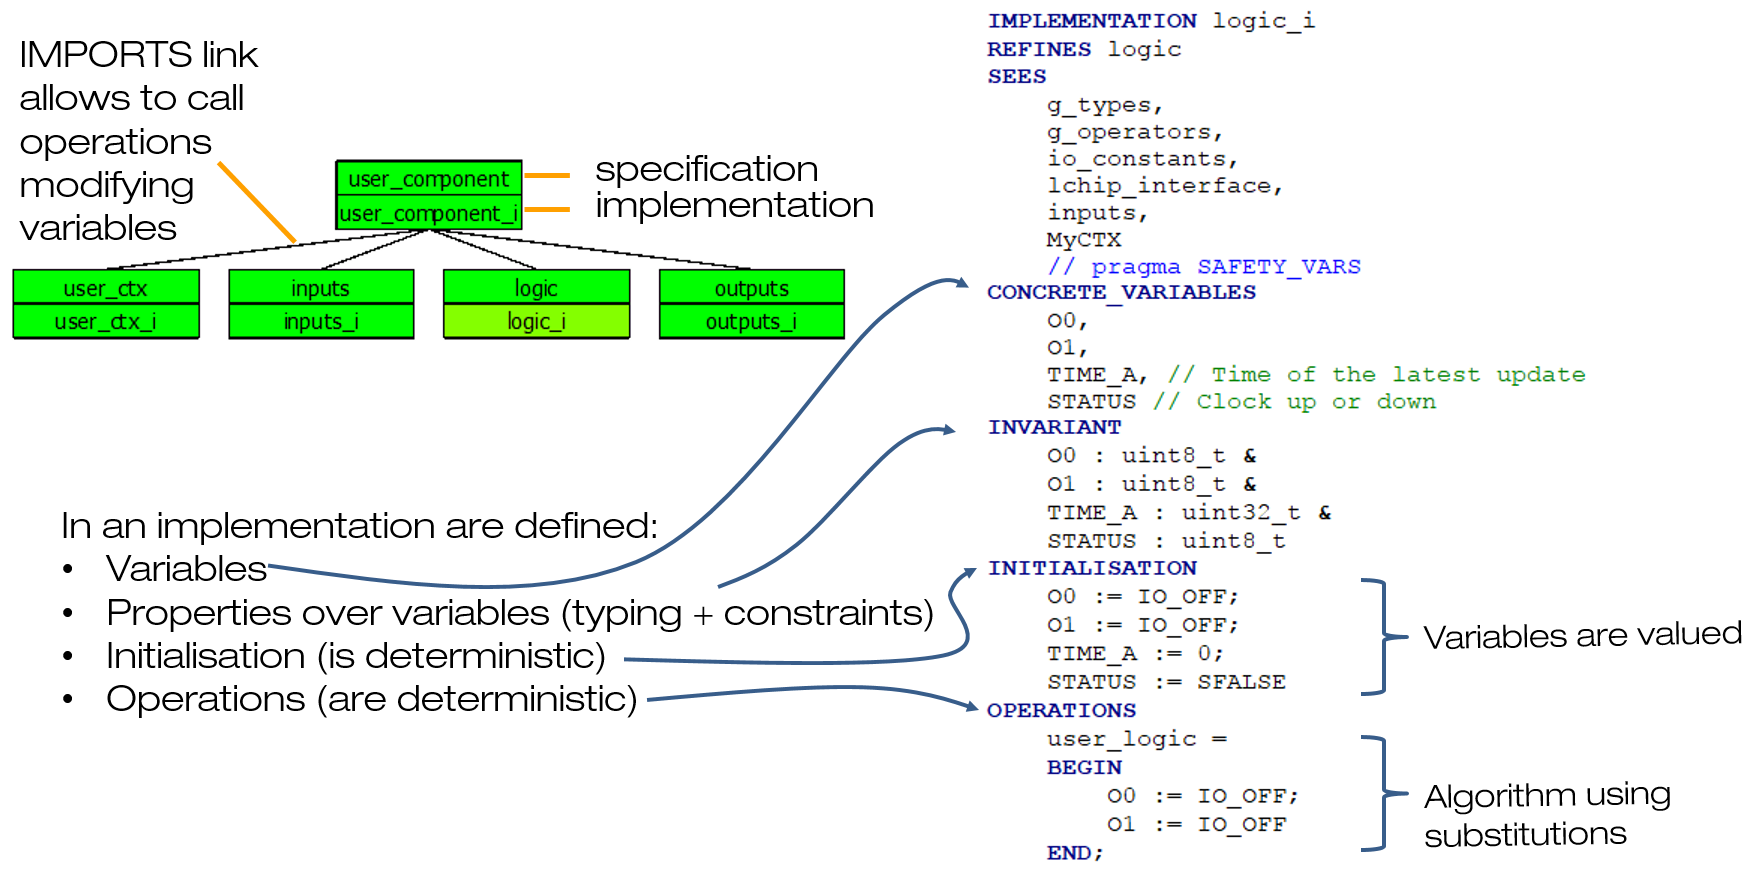
\includegraphics[scale=0.25]{Pictures/chapterProgramming/programming-implem.png}
\caption{The structure of the logic\_i component (implementation).}
\label{programming:implem}
\end{figure}  

%------------------------------------
\subsection{Declaring variables}

Figure \ref{programming:var-decl} shows how variables are declared side-by-side in specification and implementation:
\begin{itemize}
    \item first goes a list of variables, either abstract or concrete, separated by commas.
    \item in the implementation, the pragma SAFETY\_VARS is mandatory to indicate that the implementation contains variables that need to be managed by the safety library.
    \item the invariant contains a list of predicates, separated by \&, where types and constraints are expressed. Types in implementation are only implementable types.
    \item the initialisation describes the initial value of the variables. In the specification, the initialisation may be deterministic or non-deterministic. In the implementation, the initialisation has to be deterministic and to comply with the one in the specification\footnote{If "vv belongs to uint16\_t" was the initialisation of the variable vv, then "vv := 0" is a correct initialisation in implementation, while "vv := -1" is not.}. Moreover initialisations in specification are performed "in parallel" by using the operator ||; in implementation, initialisations are ordered by using the operator ; (sequence).
\end{itemize}
\begin{figure}[ht]
\centering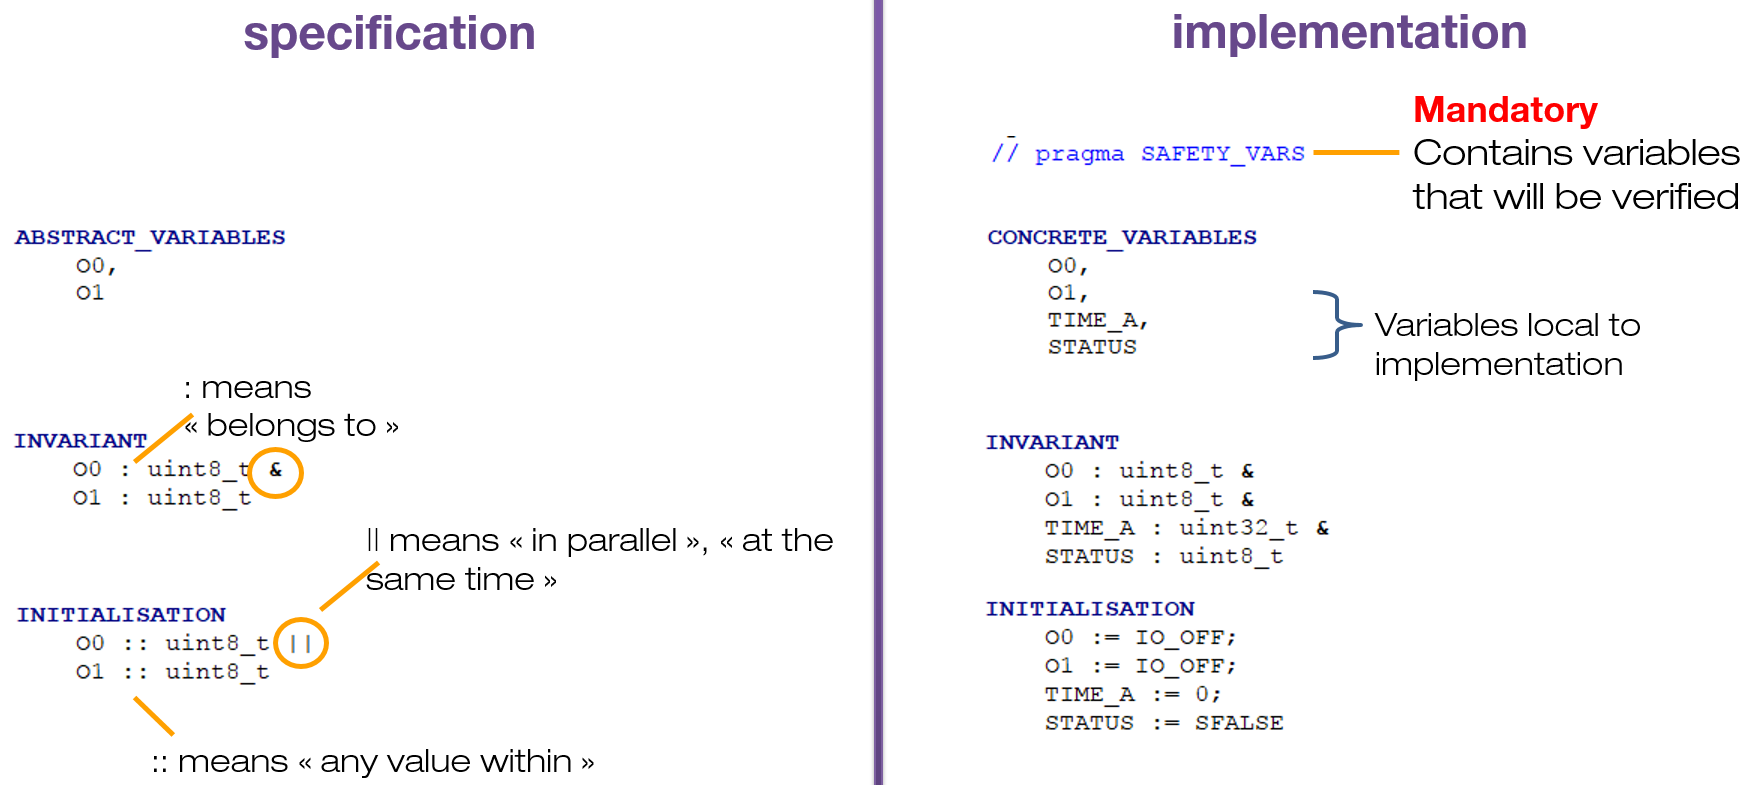
\includegraphics[scale=0.25]{Pictures/chapterProgramming/variables-decl.png}
\caption{Declaring variables in specification and implementation.}
\label{programming:var-decl}
\end{figure}  

%------------------------------------
\subsection{Declaring constants}

Figure \ref{programming:constant-decl} shows how constants are declared side-by-side in specification and implementation:
\begin{itemize}
    \item first goes a list of constants, either abstract or concrete, separated by commas.
    \item in the implementation, the pragma CONSTANTS is mandatory to indicate that the implementation contains constants that need to be managed by the safety library.
    \item in the specification, the PROPERTIES contains a list of predicates, separated by \&, where are expressed types and constraints. Properties are only in specification.
    \item in the implementation, the VALUES sets the value of the constants. Values provided have to comply with constant properties.
\end{itemize}
\begin{figure}[ht]
\centering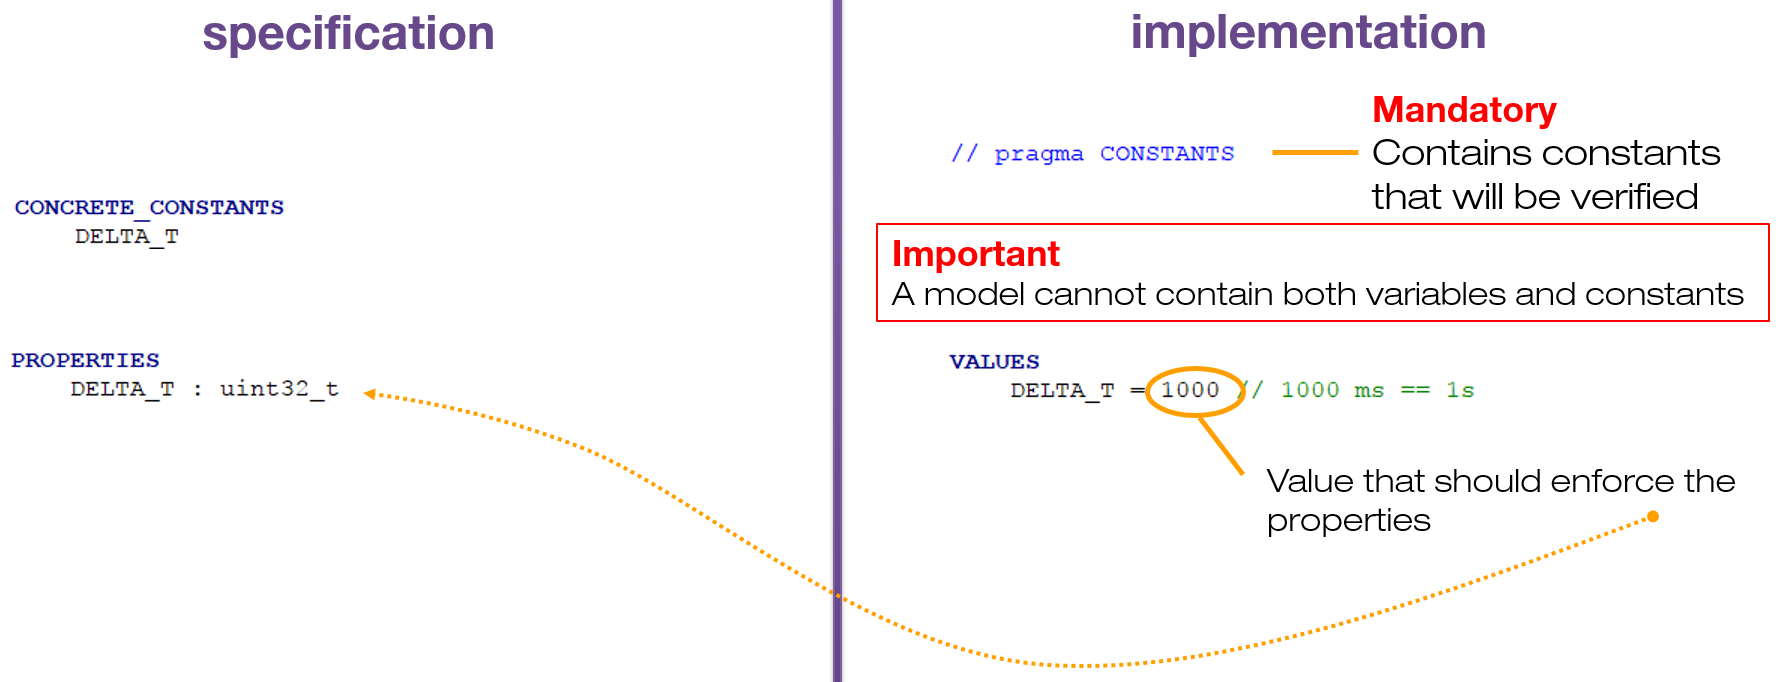
\includegraphics[scale=0.25]{Pictures/chapterProgramming/constants-decl.png}
\caption{Declaring constants in specification and implementation. }
\label{programming:constant-decl}
\end{figure}  

\begin{remark}
An implementation should contain one and only one pragma: either SAFETY\_VARS or CONSTANTS. That is why two components are made available: \textit{user\_ctx} for hosting constants and \textit{logic} for variables and behaviour.
\end{remark}

%------------------------------------
\subsection{Describing a behaviour}

Behaviour is described in OPERATIONS. Operations are populated with substitutions. Substitutions allow to describe how variables are (conditionally) modified. Available substitutions in specification are different from the ones available in implementation. We are going to see a number of these in what follows.

\subsubsection{Specification}

In specification, substitutions express the properties that the variables comply with  when the operation is completed independently from  the algorithm implemented\footnote{By using post-condition: the properties that are true when the substitution has been executed.}. A good practice is to systematically use the substitution "becomes such that" (Figure \ref{programming:subst-becomes-such-that}).\\ A simple general form of the substitution is 
\begin{center}
\textit{var : (var : type(var))}    
\end{center} where \textit{var} is an identifier and \textit{type(var)} is a set expression compatible with the type of the variable \textit{var}. It could  also be of the form:
\begin{center}
\textit{var\_list : (predicate\_list)}    
\end{center} where \textit{var\_list} is a list of identifiers separated by commas and \textit{predicate\_list} is conjunction of predicates separated by \&.
\begin{figure}[ht]
\centering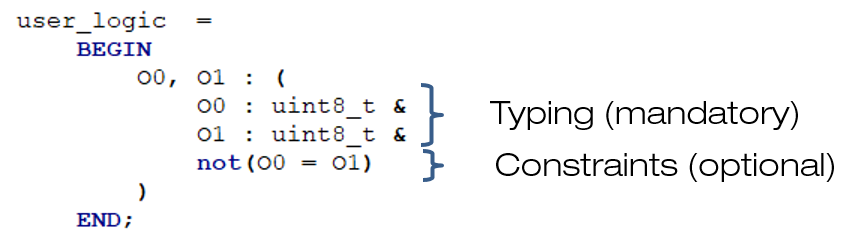
\includegraphics[scale=0.30]{Pictures/chapterProgramming/subst-becomes-such-that.png}
\caption{The substitution "becomes such that" used to specify that O0 and O1 are going to be modified within their type such that O0 is different from O1. }
\label{programming:subst-becomes-such-that}
\end{figure}  
Of course, if the value assigned to a variable is well-known, it is also possible to use the valuation substitution with:
\begin{center}
\textit{var := value}    
\end{center} where \textit{value} is a either a constant name, another variable identifier, a Boolean or an integer value.\\

If none of the variables is going to be modified then use the substitution \textit{skip}.\\

\subsubsection{Implementation}

In implementation, several substitutions are available. Some of these are shown in figure \ref{programming:subst-implem}.

\begin{figure}[ht]
\centering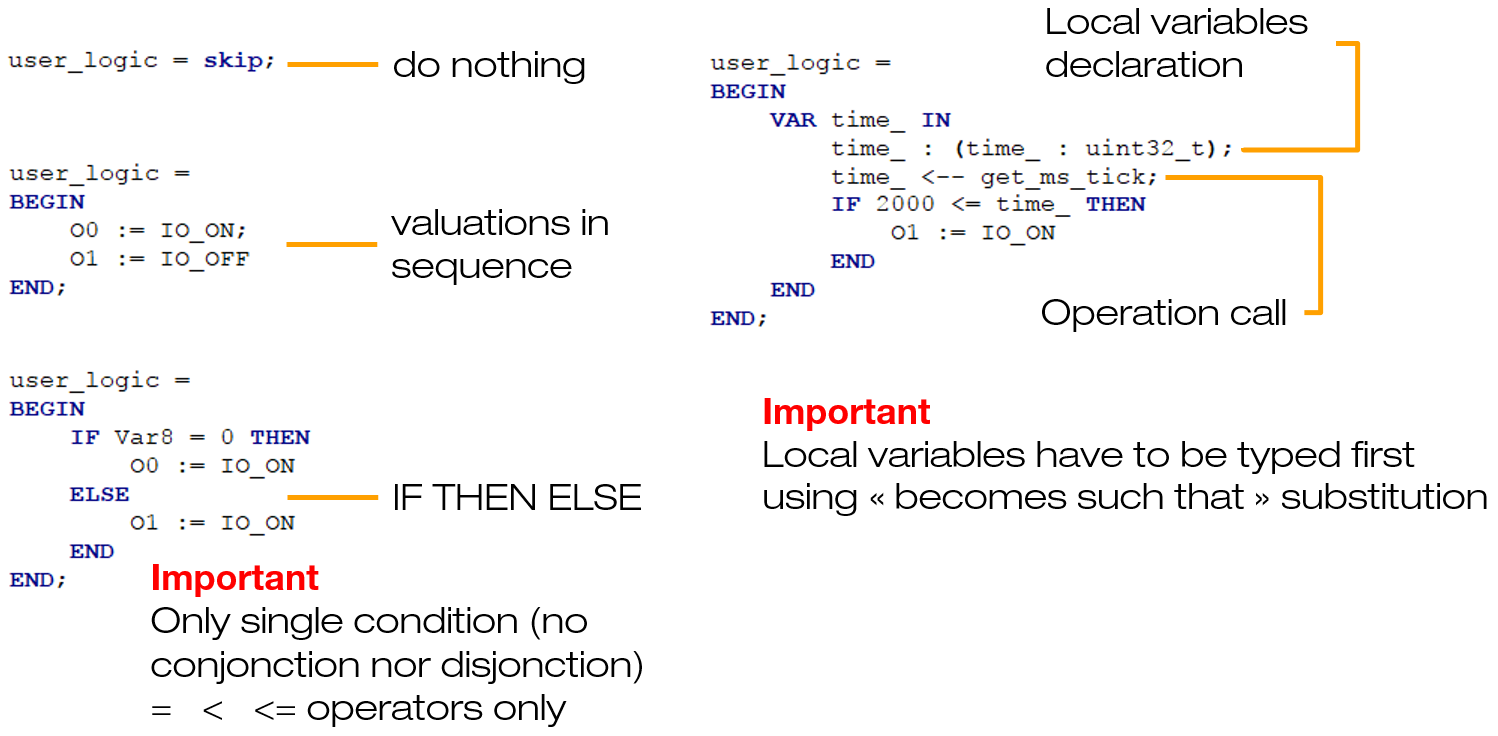
\includegraphics[scale=0.30]{Pictures/chapterProgramming/subst-implem.png}
\caption{Some substitutions usable in implementation. }
\label{programming:subst-implem}
\end{figure}  

\begin{itemize}
    \item the \textit{skip} substitution, when the variables are nor modified.
    \item the assignment substitution \textit{var := value}.
    \item the sequence substitution ; to order substitutions.
    \item the IF-THEN-ELSE substitution. Only a single condition is accepted. If several conditions have to be verified, several IF-THEN-ELSE substitutions have to be nested. Testing conditions have to be simple, hence computations have to be performed independently from (before) the test\footnote{For example, it is not possible to write IF xx+1<=yy THEN skip END. Instead a local variable has to be declared and used to compute xx+1. The test is then performed with this local variable.}
    \item the local variable substitution \textit{VAR var IN substitutions END}. Local variables are used to store data and results of computation. Before any use of a local variable a substitution "becomes such that" has to be used to give a type to this local variable.
    \item the operation call substitution \textit{var\_list <-- operation(var\_list)} which use 0..n input parameters and 0..n return parameters.
\end{itemize}
These substitutions may be used in combination to obtain the final algorithm. The loop substitution will be introduced later on, in the projects.

\subsubsection{Reconciling specification and implementation}

If the writing of an implementation is quite straightforward, especially when the logic is not too complicated, the writing of a specification is far more complex. 
\begin{figure}[ht]
\centering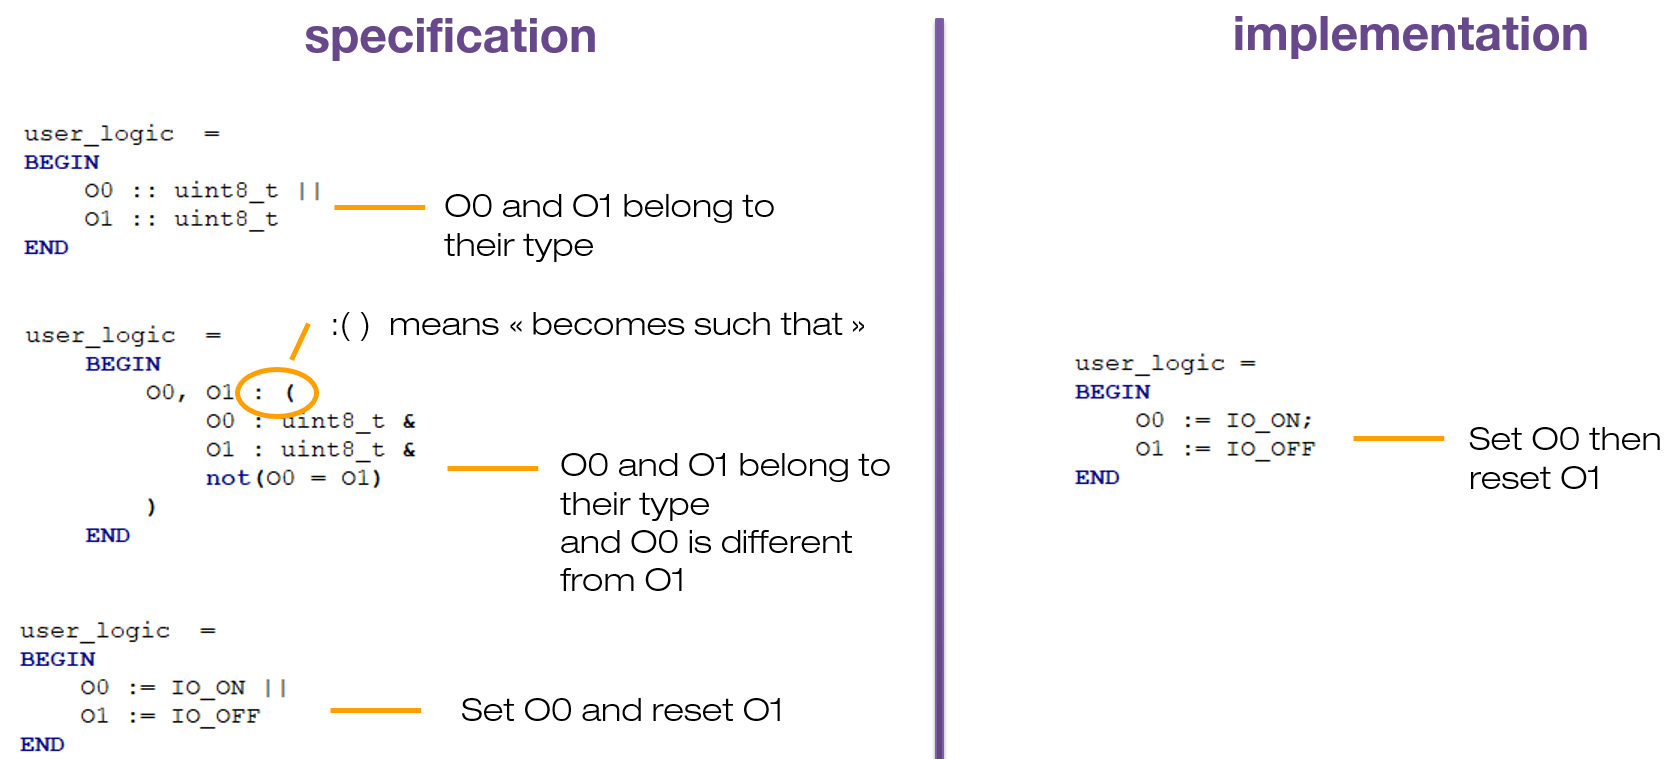
\includegraphics[scale=0.30]{Pictures/chapterProgramming/subst-reconcile.png}
\caption{Several specification compatible with the implementation. }
\label{programming:subst-reconcile}
\end{figure}  
For example, the figure \ref{programming:subst-reconcile} shows three different kinds of specification:
\begin{itemize}
    \item the first one is fully non-deterministic. If one mistake is inserted in the implementation (both values at IO\_OFF for example), it is not detected by the proof.
    \item the second one is non-deterministic but ensures that both values for O0 and O1 are different. Errors are detected except if the implementation is the contrary of what it should be.
    \item the last one is fully deterministic but very close to the specification. One risk when having such close specification/implementation is that we are only proving the copy/paste action between both models.
\end{itemize}
It is up to you to determine what kind of specification and more importantly what level of verification you are looking for. If your model only contains loosely constrained specification, the proof will not improve much the level of confidence in the algorithm.
